%!TEX root = lec05_query_processing.tex

%
% ------------------------------------------------------------------------
%
\begin{frame}{Which plan is better?}

Consider the two following plans that compute the same answer. 

They have the same I/O and memory cost. \blue{Which one will take the least \textbf{time} to execute?}

\vskip3em

\begin{center}
\begin{tikzpicture}[node distance=0.825cm,every node/.style={inner sep=1,outer sep=2,font=\footnotesize}]
    \node (1) at (0,0) {$\pi_{\texttt{director}}$};
    \node (2) [below of=1] {$\sigma_{\texttt{actor='Bill Murray'}}$};
    \node (3) [below of=2] {$\Join$};
    \node (4) [below right= of 3] {\lstinline{Movie}};
    \node (5) [below left= of 3] {\lstinline{Cast}};
    \path[commutative diagrams/.cd, every arrow, every label]
        (2) edge node {} (1)
        (3) edge node {} (2)
        (4) edge node {} (3)
        (5) edge node {} (3);   

    \tikzset{sizeEst/.style={color=red,font=\small}}
    \node [sizeEst,right of=1] {5};
    \node [sizeEst,right = 0.25cm of 2] {5};
    \node [sizeEst,right of=3] {100};
    \node [sizeEst,right of=4] {50};
    \node [sizeEst,right of=5] {100};

    \node (1) at (5,0) {$\pi_{\texttt{director}}$};
    \node (2) [below of=1] {$\Join$};
    \node (3) [below right= of 2] {\lstinline{Movie}};
    \node (4) [below left= 0.6cm and -0.125cm  of 2] {$\sigma_{\texttt{actor='Bill Murray'}}$};
    \node (5) [below of=4] {\lstinline{Cast}};
    \path[commutative diagrams/.cd, every arrow, every label]
        (2) edge node {} (1)
        (3) edge node {} (2)
        (4) edge node {} (2)
        (5) edge node {} (4);

    \tikzset{sizeEst/.style={color=red,font=\small}}
    \node [sizeEst,right of=5] {100};
    \node [sizeEst,right of=3] {50};
    \pause
    \node [sizeEst,right= 0.25cm of 4] {5};
    \pause
    \node [sizeEst,right of=2] {5};
    \node [sizeEst,right of=1] {5};
\end{tikzpicture}
\end{center}
\vskip2em
\end{frame}

%
% ------------------------------------------------------------------------
%
\begin{frame}

The previous example seems trivial: the DBMS can never do worse by performing the selection $\sigma_{\texttt{actor='Bill Murray'}}$ before the join.

\vskip1em

Sometimes the DBMS faces choices which are far from trivial.

\alert{Example 1:} if a query joins 3 tables $R, S, T$, should they be joined like this $(R\Join S)\Join T$? Or is there a better ordering?


\alert{Example 2:} if there exists a secondary index on a table, should it be used or should the DBMS scan the table instead?

\vskip2em

The next slides look into how the DBMS can choose a plan among several alternatives.

\end{frame}

%
% ------------------------------------------------------------------------
%
\begin{frame}{Result sizes and query time}

As we just saw, two plans for the same query, with the same I/O and memory cost can have different execution time, depending on the number of tuples that are computed by intermediate results.

However, the DBMS cannot execute various plans to know the exact size of their intermediate results.

\vskip1em

Instead, the DBMS needs to \textbf{estimate} those sizes for any given plan, using statistics about the database.

\begin{BOX}{Estimated vs Real Cost}
Using estimated costs, the DBMS can evaluate many candidate plans in less time than it would take to execute any of them. In practice estimated cost is correlated with actual cost.
\end{BOX}

\end{frame}

%
% ------------------------------------------------------------------------
%
\begin{frame}{Database statistics}
\label{dbms_table_statistics}
The following are the simplest statistics (per relation $R$ in the database) the DBMS can use to estimate the cost of a query plan.

\begin{center}
\begin{tabular}{rl}
$B(R)$& number of of blocks to hold all tuples in $R$ \\
$T(R)$ & number of tuples in $R$ \\
$S(R)$ & number of of bytes per tuple in $R$ \\
$V(R, a)$ & number of distinct values of $a$ in $R$
\end{tabular}
\end{center}

\vskip1em

The DBMS might also keep the lowest and the highest values of numeric attributes:

\begin{center}
\begin{tabular}{rl}
$\MIN(R, a)$ & lowest value of $a$ in $R$\\
$\MAX(R, a)$ & highest value of $a$ in $R$
\end{tabular}
\end{center}


\end{frame}

%
% ------------------------------------------------------------------------
%
\begin{frame}

\begin{columns}[onlytextwidth]
\begin{column}{0.375\textwidth}
\textbf{Example}
\vskip2em

\small
Assume:\\
- \lstinline[style=C]{sizeOf(int)} = 4 bytes\\
- \lstinline[style=C]{sizeOf(char)} = 2 bytes\\
- \lstinline[style=C]{sizeOf(float)} = 8 bytes
\end{column}
\begin{column}{0.6\textwidth}
\scalebox{0.75}{\usebox{\SimplifiedMovieTableDDL}}
\vskip1em
\scalebox{0.75}{\usebox{\MovieTable}}
\end{column}
\end{columns}

\vskip2em

\small
\begin{tabular}{l|l|l}
$T(\texttt{Movie}) = 5$ & $V(\texttt{Movie}, \texttt{title}) = 4$ & $\MIN(\texttt{Movie}, \texttt{year}) = 1984$\\
$S(\texttt{Movie}) = 92$ & $V(\texttt{Movie}, \texttt{year}) = 5$ & $\MAX(\texttt{Movie}, \texttt{year}) = 2016$\\
 & $V(\texttt{Movie}, \texttt{imdb}) = 4$ & $\MIN(\texttt{Movie}, \texttt{imdb}) = 5.3$\\
 & $V(\texttt{Movie}, \texttt{director}) = 5$ & $\MAX(\texttt{Movie}, \texttt{imdb}) = 8.1$\\
\end{tabular}
\normalsize
\end{frame}


%
%
%
\begin{frame}{Result Size Estimation}

To estimate the size of a query or sub-expression $Q$ we need to know $T(Q)$ and $S(Q)$. 

Since memory buffers have a fixed size, we can always estimate the number of buffers (and thus how much RAM) is needed as 
\[B(Q)=\ceil*{\frac{T(Q)\cdot S(Q)}{\text{buffer size}}}\]

\vskip1em

For simplicity, we consider here the cases where all tuples are of fixed size. For variable-sized tuples, the DBMS can use the average tuple size, for example, to get a reasonable estimate.

\end{frame}

%
% ------------------------------------------------------------------------
%
\begin{frame}{Estimates with Selections}

Let $Q: \sigma_{a_i=v}(R)$. 

What are good estimates for $S(Q)$ and $T(Q)$ and $V(Q,\cdot)$?
\begin{align*}
S(Q) &= S(R) \ \ \ \alert{^\dagger}\\
V(Q,a_i) &= 1 \ \ \alert{^\ddagger}\\
V(Q,a_j) &= V(R,a_j) \qquad j\neq i
\end{align*}

\vskip1em 

$\alert{^\dagger}$ Since the selection does not change the tuples.

$\alert{^\ddagger}$ For numeric attributes we can do better by checking if $\MIN(R,a_i) \leq v \leq\MAX(R,a_i)$ and assume 0 otherwise. For non-numeric attributes, such analysis is much harder.

\end{frame}


%
% ------------------------------------------------------------------------
%
\begin{frame}

What about $T(Q)$? How many tuples of $R$ should have $a_i=v$? 

\vskip1em

\begin{block}{\blue{Predicate selectivity}}
The selectivity of predicate $c_i$ is defined as \[s(R,c_i)=\frac{T(\sigma_{c_i}(R))}{T(R)}\]
and estimated as in the previous slides.
\end{block}


\vskip1em

In general, $T(\sigma_{c_i}(R)) = \ceil*{s(R, c_i)\cdot T(R)}$, for any expression $R$ (not just base tables).

\end{frame}

\begin{frame}

\textbf{\blue{Estimating} predicate selectivity}:

\vskip1em

We \alert{need to make assumptions} about how the values are distributed in order to make any estimates. 

One common assumption in cost estimation is that the values are \textbf{uniformly distributed} across the table, meaning that, for any given attribute $a_i$:
\begin{itemize}[-,topsep=-0.5em,noitemsep]
\item All $V(R,a_i)$ distinct values appear the same number of times.
\item All values are \emph{equally likely} to appear in any given tuple $t$.
\end{itemize}

\vskip2em
 
Thus:  \qquad \fbox{$s(R, \sigma_{a_i = v}) = \frac{1}{V(R, a_i)}; \qquad T(Q)= \ceil*{\frac{1}{V(R,a_i)} \cdot T(R)}$}.

\end{frame}

%
% ------------------------------------------------------------------------
%
\begin{frame}[fragile]

An alternative estimate is to assume all values \underline{in the domain} are \alert{equally likely}. This, of course, only makes sense for attributes with a discrete domain. 

In this case, we'd have $s(R, a_i=v)= \frac{1}{|\text{domain}(a_i)|}$

\vskip1em

\textbf{Example:}

\begin{center}
\begin{lstlisting}[style=SQL,basicstyle=\ttfamily\footnotesize]
CREATE TABLE Instructor(name TEXT, faculty TEXT, email TEXT, 
    CHECK (faculty IN ('Arts','Science','Engineering',
                       'Business','Law','Medicine')));
\end{lstlisting}
\end{center}

$T(\sigma_{\texttt{faculty='Arts'}}(\texttt{Instructor}))= \ceil*{\frac{1}{6} \cdot T(\texttt{Instructor})}$

\vskip1em

The estimate is always the same for values that belong to the domain, and 0 for values not in the domain.


\end{frame}


%
% ------------------------------------------------------------------------
%
\begin{frame}[fragile]{Selections With Ranges}

When the selection in based on a range of values $Q=\sigma_{a_i > v}(R)$ the estimates for $T(Q)$ and $V(Q,a_i)$ need to be adjusted.

With \emph{low}/\emph{high} statistics, we can make some reasonable estimates. If $\MIN(R,a_i)\leq v \leq \MAX(R,a_i)$\footnote{The boundary cases when $v$ is out of that range are left as an exercise.}, we can use:

\[
T(Q) = \ceil*{\frac{\MAX(R,a_i)-v}{\MAX(R,a_i)-\MIN(R,a_i)}T(R)} \text { and }\]
\[V(Q,a_i) = \ceil*{\frac{\MAX(R,a_i)-v}{\MAX(R,a_i)-\MIN(R,a_i)}V(R,a_i)}\]

Estimates for $Q=\sigma_{a_i < v}(R)$ are computed analogously.

\vskip1em

\end{frame}

%
% ------------------------------------------------------------------------
%
\begin{frame}

\textbf{Example:} $Q=\sigma_{\texttt{imdb>7} }(\texttt{Movie})$.

\[T(Q) = \ceil*{\frac{\textcolor{red}{8.1}-\alert{7}}{\textcolor{red}{8.1}-\textcolor{blue}{5.3}}\ T(\texttt{Movie})} = \ceil{1.96} =2\]

\[V(Q,\texttt{imdb}) = \ceil*{\frac{\textcolor{red}{8.1}-\alert{7}}{\textcolor{red}{8.1}-\textcolor{blue}{5.3}}\ V(\texttt{Movie},\texttt{imdb})} = \ceil{1.57} =2\]

\vskip1em

\begin{block}{}
These estimates are not great because the imdb values are \textbf{not} uniformly distributed. We would need better statistics to be more accurate here.
\end{block}

\end{frame}

%
% ------------------------------------------------------------------------
%
\newsavebox{\histogramExample}
\savebox{\histogramExample}{
    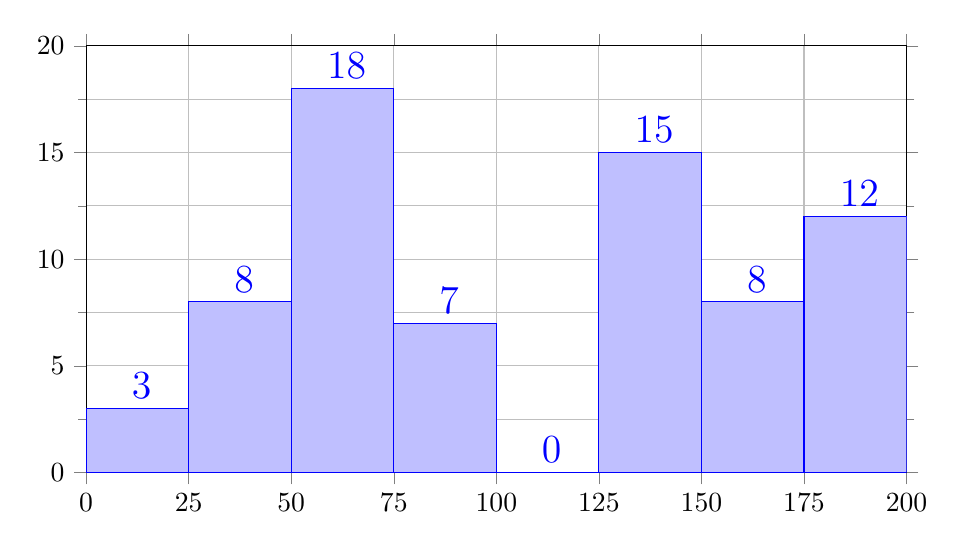
\begin{tikzpicture}
        \begin{axis}[
            height=7cm,
            width=12cm,
%            ybar interval,      % <-- this causes the `xticks' to be centered
            ymin=0,ymax=20,
            xmin=0,xmax=200,
            grid=both,
            minor y tick num=1,
            yminorgrids=true,
            xtick distance={25},
            tick align=outside, % <-- this positions the ticks "outside"
         ]
            \addplot+ [
                ybar interval,
                mark=none,
                fill=blue!25,   % fill the bars again
                nodes near coords,
                every node near coord/.append style={font=\Large,xshift=20},
            ] coordinates {
                (0,3)(25,8)(50,18)(75,7)(100,0)
                (125,15)(150,8)(175,12)
            };
            \addplot [ybar interval, % the second plot is needed to hide the
              % count of zero in the last bin.
                mark=none,
                color=blue,
                fill=blue!25,   
            ] coordinates {(175,12) (200,0)};
        \end{axis}
    \end{tikzpicture}
}

\begin{frame}{Better estimations with histograms}

\emph{Histograms} are statistical summaries of data that record the number of values that fall within predefined \textbf{bins}. 

In an \emph{equi-width} histogram, all bins have the same width, and cover the same number of elements in the domain.

\begin{center}
\scalebox{0.75}{
\begin{tikzpicture}
\node at (0,0) [anchor=north west] {\scalebox{0.5}{\usebox{\histogramExample}}};
\draw [color=accent,decorate,decoration={brace,amplitude=8pt,raise=3pt},yshift=0pt]
		(0.15,-3.15) -- (0.15,-0.25) node [midway,xshift=-1cm] {\small counts};

\draw [color=accent,decorate,decoration={brace,amplitude=8pt,raise=-3pt},yshift=0pt]
		(5.75,-3.5) -- (0.5,-3.5) node [midway,yshift=-0.35cm] {\small bins};

\draw [red] (3.75,-0.885) rectangle (4.5,-3);

\node (0) [red] at (8,-0.5) {
	\begin{minipage}{2.25cm}\baselineskip=0.75\baselineskip \centering\small
		15 values $125 \leq x <150$
	\end{minipage}
		};
\draw [red,->] (0) -- (4.56,-1);
\end{tikzpicture}}
\end{center}

We can estimate the the probability of a tuple satisfying a selection condition with a histogram of the attribute in the selection.


\end{frame}

%
% ------------------------------------------------------------------------
%
\begin{frame}

\begin{columns}[onlytextwidth]
\begin{column}{0.5\textwidth}

\[
s(R, a_i=x) = \frac{\mathit{count}(\mathit{bin}(x))}{T(R)}
\]

\vskip1em

\textbf{Examples:}
\begin{itemize}[-,noitemsep,topsep=-0.5em]
 \item $s(R, a_i=180)= 12/71$
 \item $s(R, a_i=60)= 18/71$
 \item $s(R, a_i=110)= 0$
\end{itemize}

\end{column}
\begin{column}{0.5\textwidth}
\begin{center}\scalebox{0.75}{
\begin{tikzpicture}
\node at (0,0) [anchor=north west] {\scalebox{0.5}{\usebox{\histogramExample}}};
\draw [color=accent,decorate,decoration={brace,amplitude=8pt,raise=3pt},yshift=0pt]
        (0.15,-3.15) -- (0.15,-0.25) node [midway,xshift=-1cm] {\small counts};

\draw [color=accent,decorate,decoration={brace,amplitude=8pt,raise=-3pt},yshift=0pt]
        (5.75,-3.5) -- (0.5,-3.5) node [midway,yshift=-0.35cm] {\small bins};
\end{tikzpicture}}
\end{center}
\end{column}
\end{columns}

\vskip2em

\textbf{For \alert{ranges}}, sum-up across bins overlapping with the range:
\begin{itemize}[-, noitemsep, topsep=-0.5em]
\item  $s(R, a_i \geq 100)= (0+15+8+12)/71$
\item  $s(R, 10\leq a_i <50)= (3+8)/71$
\end{itemize}

\vskip1em

For $V(Q,a_i)$ we can use either the number of values in the range (as before) or the sum of counts in the respective bins, whichever is smaller.

\end{frame}


\begin{frame}[fragile]

Histograms are an example of how \alert{better statistics offer more accurate predictions}.

The \blue{trade-off} is keeping the histogram up-to-date.
\begin{itemize}[-,topsep=-0.5em]
\item Update the histogram after every database update \textbf{or} only when the database goes offline for maintenance?
\end{itemize}

\vskip1em

\alert{What about textual attributes?}

Histograms defined by equally-spaced strings (e.g., "A", "C", "E", ...) could help with equality queries... but not \emph{wild-card queries}:

\begin{center}
\begin{lstlisting}[style=SQL]
SELECT title, imdb 
FROM Movie 
WHERE title LIKE "%space%"
\end{lstlisting}

\end{center}

Getting accurate estimates is not easy!

\end{frame}

%
% ------------------------------------------------------------------------
%
\begin{frame}

\vskip1em

What about $Q =  \alert\sigma_{\alert{c_1 \wedge \cdots \wedge c_n}}(R)$?

How many tuples satisfy \underline{all of the conditions} at the same time? This can be estimated with a bit of probability theory.

% \end{frame}

% \begin{frame}

Using $s(R, c_i)$ as the probability that a tuple in $R$ satisfies $c_i$, and assuming attribute values are \emph{independent} of each other, we have

\[
T(\sigma_{c_1 \wedge \cdots \wedge c_n}(R)) = \ceil*{\left( \prod_{1\leq i \leq n} s(R,c_i) \right) T(R)}
\]

\vskip1em

\textbf{Example:} $Q=\sigma_{\texttt{imdb>7 } \wedge \texttt{ year=2016}}(\texttt{Movie})$.

\begin{align*}
T(Q) = \ceil*{\left(\frac{2}{5} \cdot \frac{1}{5}\right) \cdot 5} = \ceil*{\frac{2}{5}} = 1
\end{align*}
\end{frame}


\begin{frame}

\vskip1em

Also using $s(R,c_i)$ as the probability that a tuple in $R$ satisfies $c_i$, and assuming attribute values are \emph{independent} of each other, we can estimate the size of a disjunction as:

\[
T(\sigma_{c_1 \vee \cdots \vee c_n}(R)) = \ceil*{\left(1 - \prod_{1\leq i \leq n} 1- s(R,c_i) \right) T(R)}
\]

The \underline{double negation} computes the probably that \alert{at least one $c_i$ is satisfied} as the complement of the probability that \emph{none} is.

\vskip1em

\textbf{Example:} $Q=\sigma_{\texttt{imdb>7 } \vee \texttt{ year=2016}}(\texttt{Movie})$.

\begin{align*}
T(Q) = \ceil*{\left(1 - \left(\frac{3}{5} \cdot \frac{4}{5}\right)\right) \cdot 5} = \ceil*{\frac{65}{25}} = 3
\end{align*}
\end{frame}


%
% ------------------------------------------------------------------------
%
\begin{frame}{Estimates with Projections}

If $Q=\pi_{a_1,\ldots,a_n}(R)$, what are good estimates for $S(Q), T(Q)$ and $V(Q,\cdot)$?
\begin{align*}
T(Q) = & T(R) \ \ \ \alert{^\dagger}\\
S(Q) = & \texttt{sizeOf}(a_1) + \cdots + \texttt{sizeOf}(a_n)\\
V(Q,a_i) = & V(R,a_i) \ \text{ if } a_i \text{ in project list}
\end{align*}

$\alert{^\dagger}$ The projection operator in SQL does not remove duplicates.

\end{frame}

%
% ------------------------------------------------------------------------
%
\begin{frame}{Estimates with Cartesian Products}

What about $Q=R_1 \times R_2$?
\begin{align*}
T(Q) = & T(R_1)T(R_2) \ \ \ \alert{^\dagger}\\
S(Q) = & S(R_1) + S(R_2) \ \ \ \alert{^\ddagger}\\
V(Q,a_i) = & \left\{\begin{array}{ll}
V(R_1,a_i) & \text{ if } a_i\in R_1\\
V(R_2, a_i) & \text{ if } a_i \in R_2
\end{array}\right.
\end{align*}

\vskip1em

$\alert{^\dagger}$ the Cartesian product produces \textbf{all pairings} of tuples.

$\alert{^\ddagger}$ the Cartesian product \textbf{concatenates} tuples together.

\end{frame}

%
% ------------------------------------------------------------------------
%
\begin{frame}{Estimates with Joins}

\alert{\textbf{Case \#1}}: A natural join $Q=R_1\Join R_2$ where $R_1$ and $R_2$ share a common attribute $a_i$.

\vskip0.5em

We immediately know that \fbox{$S(Q) = S(R_1)+S(R_2) - \texttt{sizeOf}(a_i)$} 

\vskip2em

We also know that \fbox{\alert{$0 \leq T(Q) \leq T(R_1)T(R_2)$}}... but can we get a better estimate?

\vskip0.5em

\alert{If $R_1.a_i$ is the primary key of $R_1$} and \alert{$R_2.a_i$ is a foreign key} referencing $R_1$, we know that every tuple in $R_2$ can match \blue{at most one tuple} in $R_1$, resulting in that $T(Q)=T(R_2)$.

\end{frame}


\begin{frame}

\alert{What if $a_i$ is not a key of either relation?} We need to make assumptions to estimate $T(Q)$ and $V(Q,\cdot)$.

We assume that either $R_1.a_i\subseteq R_2.a_i$ or $R_2.a_i\subseteq R_1.a_i$. That is, all values of the join attribute in the relation with the least unique values appear in the other relation\footnote{This is called the \textbf{Containment of Value Sets} Assumption.}.

\vskip1em

Then, \fbox{$V(Q,a_i) = \min\left(V(R_1, a_i), V(R_2, a_i)\right)$}.

\vskip1em

We also assume that the number of values among attributes $a_j\neq a_i$ not involved in the join are \emph{preserved}:
\[
V(Q,a_j)\ = \left\{\begin{array}{ll}
V(R_1,a_j) & \text{ if } a_j\in R_1\\
V(R_2, a_j) & \text{ if } a_j \in R_2
\end{array}\right.
\]

\end{frame}

%
% ------------------------------------------------------------------------
%
\begin{frame}

\vskip1em

To estimate $T(R_1 \Join R_2)$, consider first:

\begin{block}{How many tuples of $R_2$ will match a tuple $t\in R_1$?}
This is the same as estimating $T(\sigma_{a_i=\alert{v}}(R_2))$ where $\alert{v=t.a_i}$.
\end{block}

\vskip1em

Since \(T(\sigma_{a_i=\alert{t.a_i}}(R_2)) = \ceil*{\frac{1}{V(R_2, a_i)}\cdot T(R_2)}\), and since we assumed that \blue{every tuple} in $R_1$ will match at least one tuple in $R_2$, we have:

\[T(R_1 \Join R_2) = \ceil*{\alert{T(R_1)}\cdot\frac{T(R_2)}{V(R_2,a_i)}}\]

\end{frame}

\begin{frame}

Swapping $R_1$ and $R_2$ in the analysis above gives another estimate:

\[T(R_1 \Join R_2) = \ceil*{\alert{T(R_2)}\cdot\frac{T(R_1)}{V(R_1,a_i)}}\]

\vskip2em

If the two estimates disagree, we take the least of them, arriving at

\[
T(Q) = \ceil*{\frac{T(R_1)T(R_2)}{\alert{\max}(V(R_1,a_i), V(R_2,a_i))}}
\]
\end{frame}



\begin{frame}

Because a join is equivalent to a Cartesian product followed by a selection

\[R_1 \Join_c R_2 = \sigma_c (R_1 \times R_2)\]

\vskip1em

And because we assume that \(T(\sigma_c(R) = \ceil*{s(R, c)T(R)}\), we arrive at an expression for the selectivity of an equality predicate in a join:

\[
s(R_1 \times R_2, R_1.a_i = R_2.a_i) = \frac{1}{\max(V(R_1,a_i), V(R_2,a_i))}
\]

\end{frame}


%
% ------------------------------------------------------------------------
%
\begin{frame}

\vskip1em


Let $Q=R_1(a,b,c) \Join_{a=d} R_2(d,e)$. 

In this case, note that there are no attributes in common, so \[S(Q) = S(R_1) + S(R_2)\]

\vskip1em

But what will be a good estimate for $T(Q)$?

A similar analysis as in the case of the natural gives:

\[
s(R_1 \times R_2, R_1.a = R_2.d) = \frac{1}{\max(V(R_1,a), V(R_2,d))}
\]

Therefore:

\[T(Q)=\ceil*{\frac{T(R_1)T(R_2)}{\alert{\max}(V(R_1,a),V(R_2,d))}}\]

\end{frame}

\begin{frame}

\vskip1em

If the join has many predicates, they are treated as \emph{independent} events. 


Let $Q=R_1(a,b,c) \Join_{a=d \, \wedge \, c=e} R_2(d,e)$. Then:

\(
s(R_1 \times R_2, R_1.a = R_2.d) = \frac{1}{\max(V(R_1,a), V(R_2,d))}
\)

\(
s(R_1 \times R_2, R_1.c = R_2.e) = \frac{1}{\max(V(R_1,c), V(R_2,e))}
\)

And:


\[T(Q)=\ceil*{\frac{T(R_1)T(R_2)}{\alert{\max}(V(R_1,a),V(R_2,d)) \cdot \alert{\max}(V(R_1,c)),(V(R_2,e))}}\]
\end{frame}

%
% ------------------------------------------------------------------------
%
\begin{frame}
Let $Q=R_1\Join R_2 \Join R_3$, where all three relations have attribute $a$ in common. In this case, treat the joins $R_1\Join R_2$ and $R_2 \Join R_3$ as independent events, arriving at:

\[T(Q)=\ceil*{\frac{T(R_1)T(R_2)T(R_3)}{\alert{\max}(V(R_1,a),V(R_2,a)) \cdot \alert{\max}(V(R_2,a)),(V(R_3,a))}}\]

\vskip2em

In general, for $Q=R_1 \Join R_2 \Join \cdots \Join R_k$, we estimate $T(Q)$ by finding the selectivity of the pairwise join conditions and using their \textbf{product} for the final selectivity of the multi-way join as a whole.

Again, we do this because we assume that the events corresponding to tuples joining are independent of one another.

\end{frame}



\begin{frame}{Other Estimates...}

For joins with disjunctions $R_1 \Join_{c_1 \vee \cdots \vee c_n} R_2$ we can use the ``complement of the complements'' method to find the selectivity of the entire join predicate.

For conditions defined with inequalities $R_1 \Join_{a > b} R_2$, we can adapt ideas from predicate selectivity estimation for selections to find the selectivity.

\vskip2em

The size of queries with \textbf{aggregations} is determined by the number of groupings that exist in the table. 

Using $V(R,a_i)$ for each attribute $a_i$ in the grouping set, we can estimate the total number of groups, again assuming attributes are independent of one another.
\end{frame}


\begin{frame}

What about set operations?

Reliable estimates are possible for \textbf{set operations} that can be rewritten as conjunctions or disjunctions:
\begin{itemize}[-,topsep=-0.5em,noitemsep]
\item recall $\sigma_{c_1} (R) \cup \sigma_{c_2} (R) = \sigma_{c_1 \vee c_2} (R)$ and
\item $\sigma_{c_1} (R) \cap \sigma_{c_2} (R) = \sigma_{c_1 \wedge c_2} (R)$
\end{itemize}

\vskip2em

If that's not possible, we can at least get \emph{upper bounds} on $T(Q)$:
\begin{center}
\begin{align*}
T(R \cup S) &= T(R) + T(S)\\
T(R \cap S) &= \min(T(R), T(S))\\
T(R - S) &= T(R)
\end{align*}
\end{center}

\end{frame}
